\documentclass[aspectratio=169]{../latex_main/tntbeamer}  % you can pass all options of the beamer class, e.g., 'handout' or 'aspectratio=43'
\usepackage{dsfont}
\usepackage{bm}
\usepackage[english]{babel}
\usepackage[T1]{fontenc}
%\usepackage[utf8]{inputenc}
\usepackage{graphicx}
\graphicspath{ {./figures/} }
\usepackage{algorithm}
\usepackage[ruled,vlined,algo2e,linesnumbered]{algorithm2e}
\usepackage{hyperref}
\usepackage{booktabs}
\usepackage{mathtools}

\usepackage{amsmath,amssymb}

\DeclareMathOperator*{\argmax}{arg\,max}
\DeclareMathOperator*{\argmin}{arg\,min}

\usepackage{amsbsy}
\newcommand{\vect}[1]{\bm{#1}}
%\newcommand{\vect}[1]{\boldsymbol{#1}}

\usepackage{pgfplots}
\pgfplotsset{compat=1.16}
\usepackage{tikz}
\usetikzlibrary{trees} 
\usetikzlibrary{shapes.geometric}
\usetikzlibrary{positioning,shapes,shadows,arrows,calc,mindmap}
\usetikzlibrary{positioning,fadings,through}
\usetikzlibrary{decorations.pathreplacing}
\usetikzlibrary{intersections}
\pgfdeclarelayer{background}
\pgfdeclarelayer{foreground}
\pgfsetlayers{background,main,foreground}
\tikzstyle{activity}=[rectangle, draw=black, rounded corners, text centered, text width=8em]
\tikzstyle{data}=[rectangle, draw=black, text centered, text width=8em]
\tikzstyle{myarrow}=[->, thick, draw=black]

% Define the layers to draw the diagram
\pgfdeclarelayer{background}
\pgfdeclarelayer{foreground}
\pgfsetlayers{background,main,foreground}

% Requires XeLaTeX or LuaLaTeX
%\usepackage{unicode-math}

\usepackage{fontspec}
%\setsansfont{Arial}
\setsansfont{RotisSansSerifStd}[ 
Path=../latex_main/fonts/,
Extension = .otf,
UprightFont = *-Regular,  % or *-Light
BoldFont = *-ExtraBold,  % or *-Bold
ItalicFont = *-Italic
]
\setmonofont{Cascadia Mono}[
Scale=0.8
]

% scale factor adapted; mathrm font added (Benjamin Spitschan @TNT, 2021-06-01)
%\setmathfont[Scale=1.05]{Libertinus Math}
%\setmathrm[Scale=1.05]{Libertinus Math}

% other available math fonts are (not exhaustive)
% Latin Modern Math
% XITS Math
% Libertinus Math
% Asana Math
% Fira Math
% TeX Gyre Pagella Math
% TeX Gyre Bonum Math
% TeX Gyre Schola Math
% TeX Gyre Termes Math

% Literature References
\newcommand{\lit}[2]{\href{#2}{\footnotesize\color{black!60}[#1]}}

%%% Beamer Customization
%----------------------------------------------------------------------
% (Don't) Show sections in frame header. Options: 'sections', 'sections light', empty
\setbeamertemplate{headline}{empty}

% Add header logo for normal frames
\setheaderimage{
	% 
\includegraphics[height=\logoheight]{figures/TNT_darkv4.pdf}
	
\includegraphics[height=\logoheight]{../latex_main/figures/luh_logo_rgb_0_80_155.pdf}
	% 
\includegraphics[height=\logoheight]{figures/logo_tntluh.pdf}
}

% Header logo for title page
\settitleheaderimage{
	% 
\includegraphics[height=\logoheight]{figures/TNT_darkv4.pdf}
	
\includegraphics[height=\logoheight]{../latex_main/figures/luh_logo_rgb_0_80_155.pdf}
	% 
\includegraphics[height=\logoheight]{figures/logo_tntluh.pdf}
}

% Title page: tntdefault 
\setbeamertemplate{title page}[tntdefault]  % or luhstyle
% Add optional title image here
%\addtitlepageimagedefault{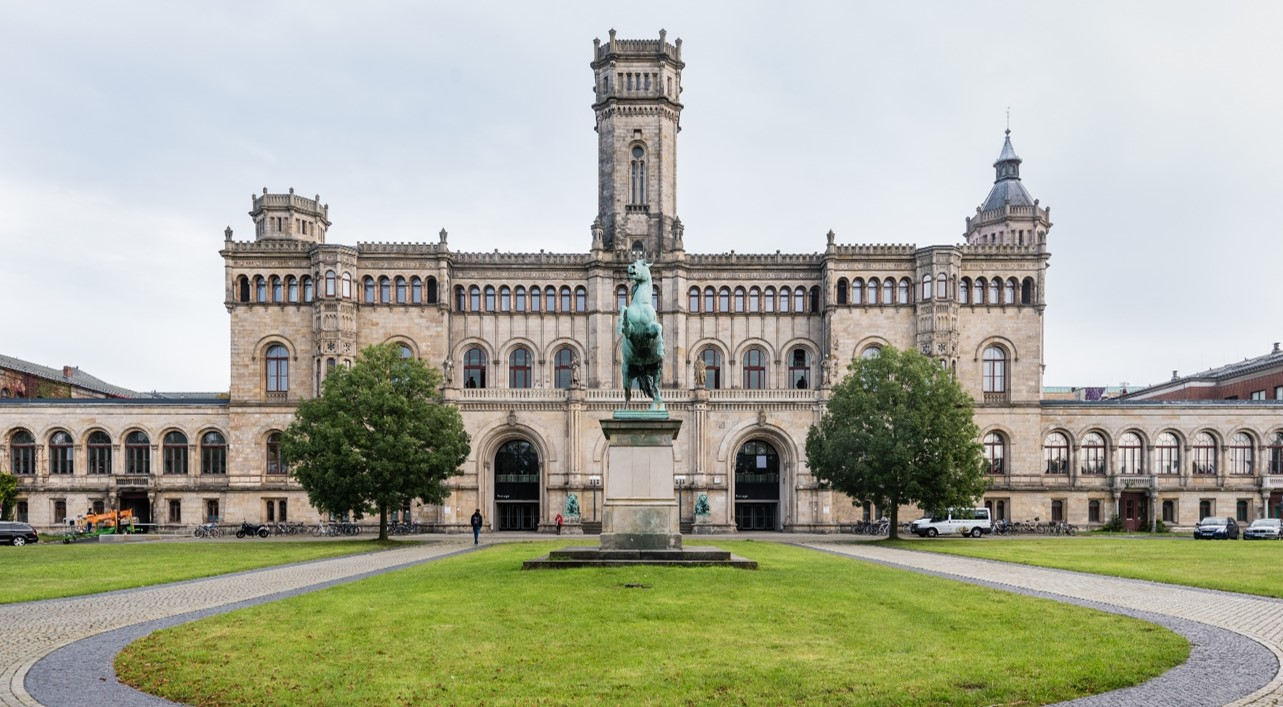
\includegraphics[width=0.65\textwidth]{figures/luh_default_presentation_title_image.jpg}}

% Title page: luhstyle
% \setbeamertemplate{title page}[luhstyle]
% % Add optional title image here
% \addtitlepageimage{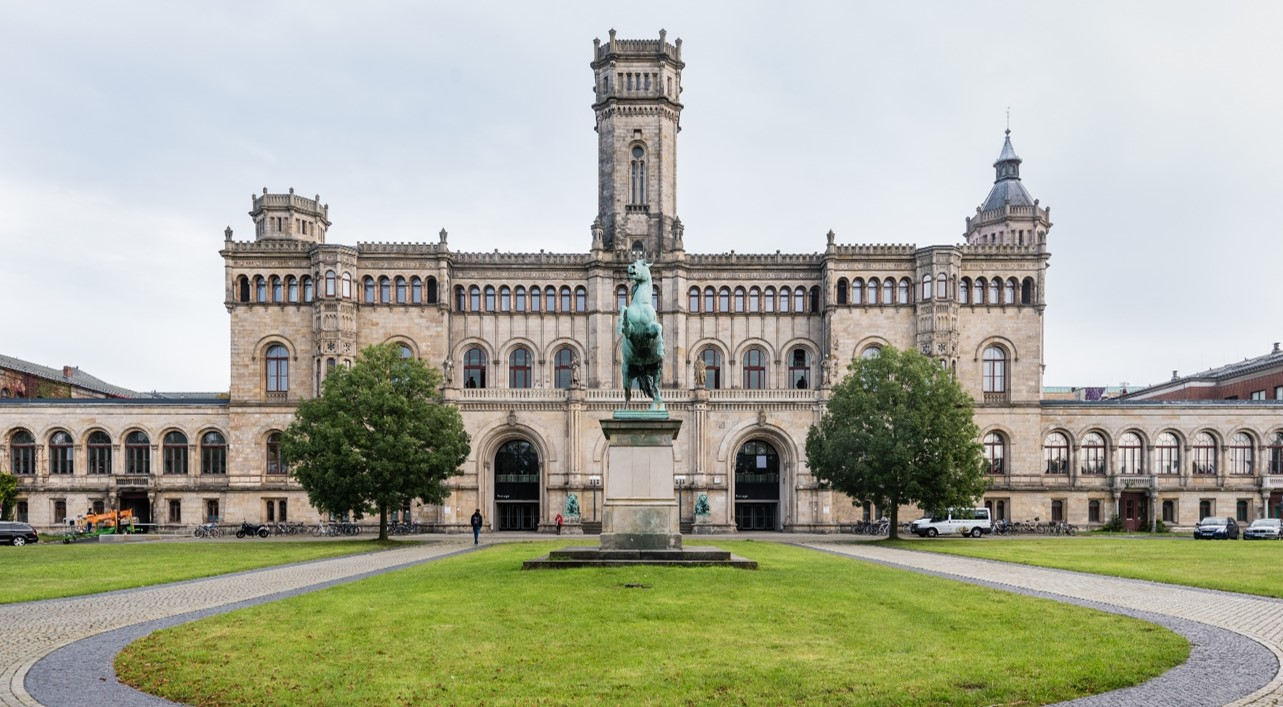
\includegraphics[width=0.75\textwidth]{figures/luh_default_presentation_title_image.jpg}}

\author[Abedjan \& Lindauer]{Ziawasch Abedjan \& Marius Lindauer\\[1em]
	
\includegraphics[height=\logoheight]{../latex_main/figures/luh_logo_rgb_0_80_155.pdf}\qquad
	
\includegraphics[height=\logoheight]{../latex_main/figures/DBIS_Kurzlogo.png}\qquad

\includegraphics[height=\logoheight]{../latex_main/figures/TNT_darkv4}\qquad

\includegraphics[height=\logoheight]{../latex_main/figures/L3S.jpg}	}
\date{Summer Term 2022; \hspace{0.5em} {
\includegraphics[height=1.5em]{../latex_main/figures/Cc-by-nc-sa_icon.svg.png}}; based on \href{https://ds100.org/fa21/}{[DS100]}
}


%%% Custom Packages
%----------------------------------------------------------------------
% Create dummy content
\usepackage{blindtext}

% Adds a frame with the current page layout. Just call \layout inside of a frame.
\usepackage{layout}


%%% Macros
%\renewcommand{\vec}[1]{\mathbf{#1}}
% \usepackage{bm}
%\let\vecb\bm

\title[Regression]{DS: Ordinary Least Squares}
\subtitle{Linear algebra formulation}

\graphicspath{ {./figure_ols/} }
%\institute{}


\begin{document}
	
	\maketitle
	\begin{frame}{Dot products}
	    The dot product of two vectors 		$\vect{a} = \left[\begin{array}{c}
	          a_1 \\
	          a_2 \\
	          \vdots\\
	          a_n
	    \end{array}\right]$	       and	$\vect{b} = \left[\begin{array}{c}
	          b_1 \\
	          b_2 \\
	          \vdots\\
	          b_n
	    \end{array}\right]$			   is defined as follows: 
	    \begin{equation*}
	        \vect{a} \cdot \vect{b} = a_1b_1 + a_2b_2 + \dots + a_nb_n
	    \end{equation*}
	   
    \begin{itemize}
        \item An alternate way of writing a dot product: $\vect{a}\cdot \vect{b} = \vect{a}^\intercal \vect{b}$
        \begin{itemize}
            \item This is the form we will use primarily moving forward.
        \end{itemize}
            \item The dot product between two vectors is a scalar, not another vector.
            \item The dot product is only defined for two vectors of the same length.  
           % \item The dot product is a special case of the inner product.
    \end{itemize}

	\end{frame}
	
	
	\begin{frame}{Multiple regression as a dot product}
	   We previously stated that the multiple regression model was of the form\\
        \hspace{3cm}
	    $\hat{y} = f_\theta (\vect{x}) = \theta_0 + \theta_1x_1 + \theta_2x_2 + ... + \theta_px_p = \sum\limits_{j=1}^p\theta_jx_j$ 
	   
	   This can be restated as a dot product between two vectors.

	   	$\vect{\theta} = \left[\begin{array}{c}
	          \theta_0\\
	          \theta_1 \\
	          \theta_2 \\
	          \vdots\\
	          \theta_p
	    \end{array}\right]$	       
	    $\vect{x} = \left[\begin{array}{c}
	          1\\
	          x_1 \\
	          x_2 \\
	          \vdots\\
	          x_p
	    \end{array}\right]$	\\
	    \bigskip
	    $\leadsto$ $\hat{y} = \vect{x}^\intercal\vect{\theta}$\\[2em]
	    
	    \alert{Note}: Letter is either \textbf{boldface} (i.e. vector, matrix, tensor) or not (scalar)
	    
	\end{frame}
	
	
	\begin{frame}{Design matrix}
	\begin{itemize}
	    \item Consider all observations at once
	    \item[$\leadsto$] express our model in terms of all observations (instead of a single observation)
	    \item Let's define a design matrix with all $n$ observations (and $p$ features):
	\end{itemize}
	  \begin{align*}
	       \vect{X} = \left[\begin{array}{cccccc}
	          1 & x_{11} & x_{12} & x_{13} & \dots & x_{1p}\\
	          1 & x_{21} & x_{22} & x_{23} & \dots & x_{2p}\\
	          1 & x_{31} & x_{32} & x_{33} & \dots & x_{3p}\\
	          \vdots     & \vdots & \vdots &\vdots &  \vdots \\
	          1 & x_{n1} & x_{n2} & x_{n3} & \dots & x_{np}\\
	    \end{array}\right]
	  \end{align*}
	  Rows correspond to observations. e.g. all features for data point 3\\
	  Columns correspond to features.  e.g. feature 1, for all data points
	\end{frame}
	
	
	\begin{frame}{Example design matrix}
	
	  \begin{columns}
	  
	      \begin{column}{.5\textwidth}
	      
	            \centering
	            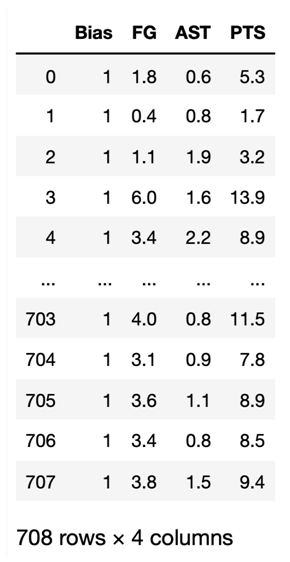
\includegraphics[scale=.4]{Bild1}
	            
	      \end{column}
	      
	      \begin{column}{.4\textwidth}
	      
	            Here, n = 708, and p = 3.
	            
	            \begin{itemize}
	                \item Each of the 4 columns corresponds to a different feature.
	                \item Each of the 708 rows corresponds to a different data point.
	            \end{itemize}
	            
	      \end{column}
	      
	  \end{columns}
	  
	\end{frame}
	
	\begin{frame}{Multiple regression as a matrix multiplication}
	    This allows us to express our linear model on our entire dataset (not just one observation) as
	    \begingroup
	    \Large
        \begin{equation*}
            \hat{\vect{Y}} = \vect{X}\vect{\theta}
        \end{equation*}
        \endgroup
        $\hat{\vect{Y}}$: Vector with dimensions $n \times 1$.\\
        $\vect{X}$: Matrix with dimensions $n \times (p + 1)$.\\
        $\vect{\theta}$: Vector with dimensions $(p + 1) \times 1$\\
        \bigskip
        Note: This means that $\vect{Y}$  represents an n-length vector containing all of our true $y$ values.
	\end{frame}
	
	
	\begin{frame}{Multiple regression as a matrix multiplication}
	  \begin{align*}
	       \left[\begin{array}{c}
	          \hat{y_1}\\ 
	          \hat{y_2}\\ 
	          \hat{y_3}\\ 
	          \vdots  \\
	          \hat{y_n}\\ 
	    \end{array}\right] = \left[\begin{array}{cccccc}
	          1 & x_{11} & x_{12} & x_{13} & \dots & x_{1p}\\
	          1 & x_{21} & x_{22} & x_{23} & \dots & x_{2p}\\
	          1 & x_{31} & x_{32} & x_{33} & \dots & x_{3p}\\
	          \vdots     & \vdots & \vdots &\vdots &  \vdots \\
	          1 & x_{n1} & x_{n2} & x_{n3} & \dots & x_{np}\\
	    \end{array}\right]
	    \left[\begin{array}{c}
	          \theta_0\\
	          \theta_1\\ 
	          \theta_2\\ 
	          \theta_3\\ 
	          \vdots  \\
	          \theta_p\\ 
	    \end{array}\right]
	  \end{align*}
	  Moving forward:

	  \begin{itemize}
	      \item    $\vect{X}_{i,:}$ or just simply $\vect{X}_{i}$ will represent row i of our design matrix.\\ Rows are observations / data points.
          \item   $\vect{X}_{:,j}$ will represent column j of our design matrix. Columns are features.

	  \end{itemize}
	\end{frame}
	
	
	\begin{frame}{Multiple regression as a matrix multiplication}
	  \begin{align*}
	       \left[\begin{array}{c}
	          \hat{y_1}\\ 
	          \hat{y_2}\\ 
	          \hat{y_3}\\ 
	          \vdots  \\
	          \hat{y_n}\\ 
	    \end{array}\right] = \left[\begin{array}{cccccc}
	          1 & x_{11} & x_{12} & x_{13} & \dots & x_{1p}\\
	          \alert{1} & \alert{x}_{21} & \alert{x}_{22} & \alert{x}_{23} & \alert{\dots} & \alert{x}_{2p}\\
	          1 & x_{31} & x_{32} & x_{33} & \dots & x_{3p}\\
	          \vdots     & \vdots & \vdots &\vdots &  \vdots \\
	          1 & x_{n1} & x_{n2} & x_{n3} & \dots & x_{np}\\
	    \end{array}\right]
	    \left[\begin{array}{c}
	          \theta_0\\
	          \theta_1\\ 
	          \theta_2\\ 
	          \theta_3\\ 
	          \vdots  \\
	          \theta_p\\ 
	    \end{array}\right]
	  \end{align*}
	  For instance, to compute the predicted output for the second observation:
        \begin{equation*}
            \hat{y}_2 = \theta_0 + \theta_1x_{21} + \theta_2x_{22} + \theta_3x_{23} + ... + \theta_px_{2p}
        \end{equation*}
        Or, more compactly:
        \begin{equation*}
            \hat{y_2} = \vect{X}_2^\intercal \vect{\theta}
        \end{equation*}
        $\vect{X}_2$ is a vector, not a matrix. That is why it is transposed.

	\end{frame}
	
	
	\begin{frame}{Example}
	    \begin{columns}
	        \begin{column}{.4\textwidth}
	              Consider the following design matrix and value of $\vect{\theta}$.
	              \begin{figure}
	                  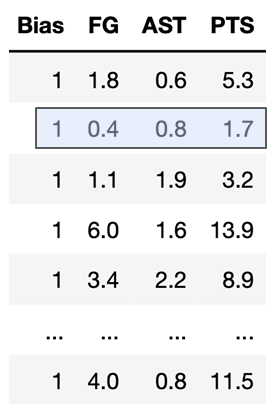
\includegraphics[scale=.35]{Bild2}
	                   $\vect{\theta} = \left[\begin{array}{r}
	                   -5  \\
	                   2 \\
	                   -1 \\
	                   3
	              \end{array}\right]$
	              \end{figure}
	        \end{column}
	        
	        
	         \begin{column}{.4\textwidth}
	              The predicted response (output) for the second observation:
	                \begin{align*}
	                   \hat{\vect{y}_2} &=[1, 0.4, 0.8 ,1.7] \cdot \left[\begin{array}{r}
	                   -5  \\
	                   2 \\
	                   -1 \\
	                   3
	                   \end{array}\right]\\
	                      &= 1(-5)+0.4(2)+0.8(-1) + 1.7(3)\\
	                      &=0.1
	                 \end{align*}
	                   
	                  
	        \end{column}
	    \end{columns}
	\end{frame}
	
	
% 	\begin{frame}{Example}
% 	    \begin{columns}
% 	        \begin{column}{.4\textwidth}
% 	              Consider the following design matrix and value of $\theta$.
% 	              \begin{figure}
% 	                  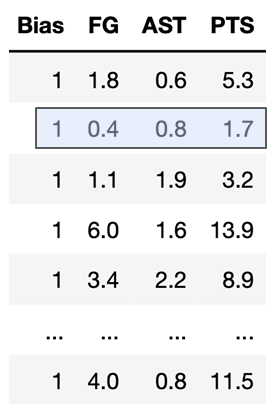
\includegraphics[scale=.35]{Bild2}
% 	                   $\theta = \left[\begin{array}{}
% 	                   -5  \\
% 	                   2 \\
% 	                   -1 \\
% 	                   3
% 	              \end{array}\right]$
% 	              \end{figure}
% 	        \end{column}
	        
	        
% 	         \begin{column}{.4\textwidth}
% 	              The predicted response 
% 	                \begin{figure}
% 	                    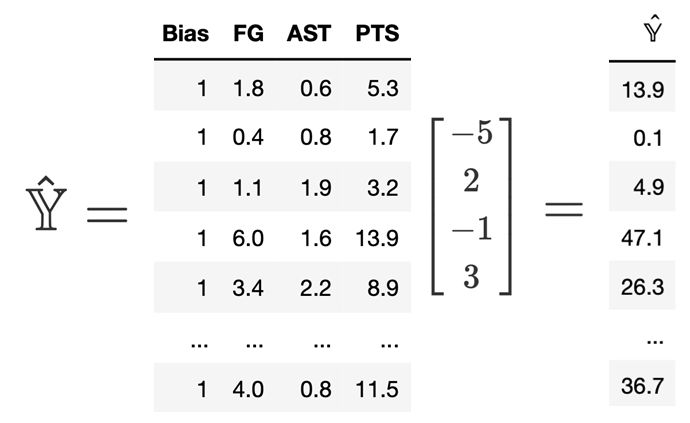
\includegraphics[scale=0.35]{Bild3}
% 	                \end{figure}
	                   
	                  
% 	        \end{column}
% 	    \end{columns}
% 	\end{frame}
	
	
	\begin{frame}{Summary of notation}
	    \begin{columns}
	        \begin{column}{.4\textwidth}
	              When looking at a single observation, our model is
	              \begin{equation*}
	                  \hat{y} = f_{\vect{\theta}} (\vect{x}) = \vect{x}^\intercal\vect{\theta}
	              \end{equation*}
	              
	              \begin{itemize}
	                  \item $\vect{x}$ is a vector of size $p + 1$.
	                  \item $\hat{y}$     is a scalar.
	                  \item $\vect{\theta}$     is a vector of size $p + 1$.
	              \end{itemize}
	        \end{column}
	        
	        
	         \begin{column}{.45\textwidth}
	             When looking at multiple observations, our model is
	              \begin{equation*}
	                  \hat{\vect{Y}} = \vect{X}\vect{\theta }
	              \end{equation*}
	              
	              \begin{itemize}
	                  \item $\vect{X}$ is a matrix of size $n \times (p + 1)$.
	                  \item $\hat{\vect{Y}}$ is a vector of size $n$ (i.e.  $\hat{\vect{Y}} \in \mathbb{R}^n$).
	                  \item $\vect{\theta}$ is a vector of size $p + 1$.
	              \end{itemize}
	        \end{column}
	    \end{columns}
	    \bigskip
	    In many settings, we assume that we have only $p$ (and not $p + 1$) columns. One of those $p$ columns may be “1” for each observation.
	\end{frame}
\end{document}